\documentclass{article}

\usepackage[utf8]{inputenc}
\usepackage{graphicx}
\usepackage{amsmath}
\usepackage{amsfonts}
\usepackage{amssymb}
\usepackage{comment}
\usepackage{gensymb}
\usepackage{geometry}
\usepackage{float}
\usepackage{caption}
\usepackage{subcaption}
\usepackage{listings}
\usepackage{enumitem}

\geometry{a4paper, margin=1in}

\lstset{
    basicstyle=\ttfamily\small,
}

\title{CSCE 312 Lab 3}
\author{Kevin Lei}
\date{February 25, 2024}


\begin{document}

\maketitle

\section*{Problem 1}
Here we implement a D flip-flop from scratch using only NAND gates.
The D flip-flop uses two D latches, which are implemented as follows:
\begin{figure}[H]
    \centering
    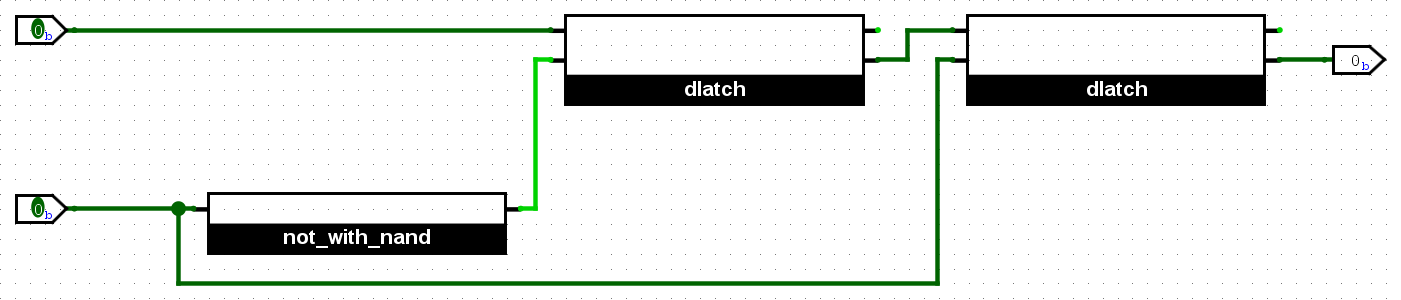
\includegraphics[width=0.9\textwidth]{./images/d_flip_flop.png}
    \caption{D Flip-Flop}
\end{figure}

\noindent The D latches are implemented as follows:
\begin{figure}[H]
    \centering
    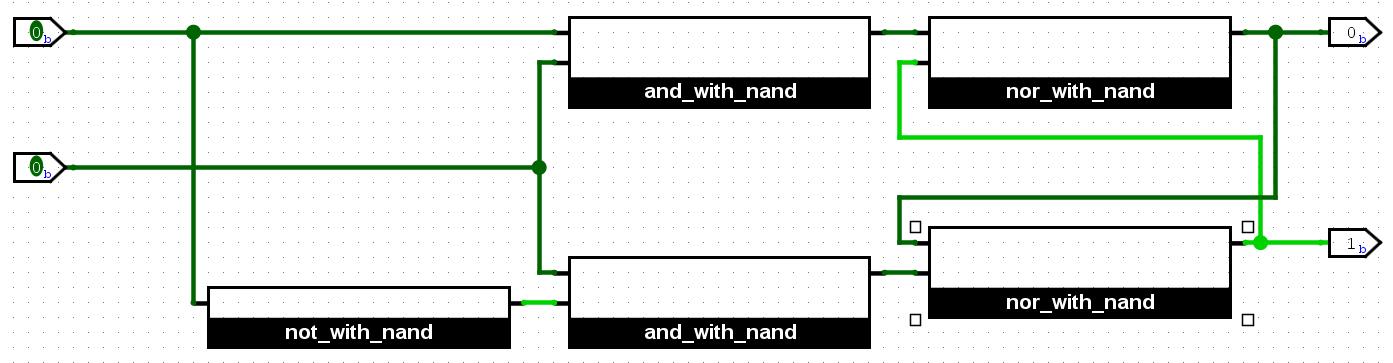
\includegraphics[width=0.9\textwidth]{./images/d_latch.png}
    \caption{D Latch}
\end{figure}

\noindent The NOR, NOT, and AND gates are implemented as follows:
\begin{figure}[H]
    \begin{minipage}{0.5\textwidth}
        \centering
        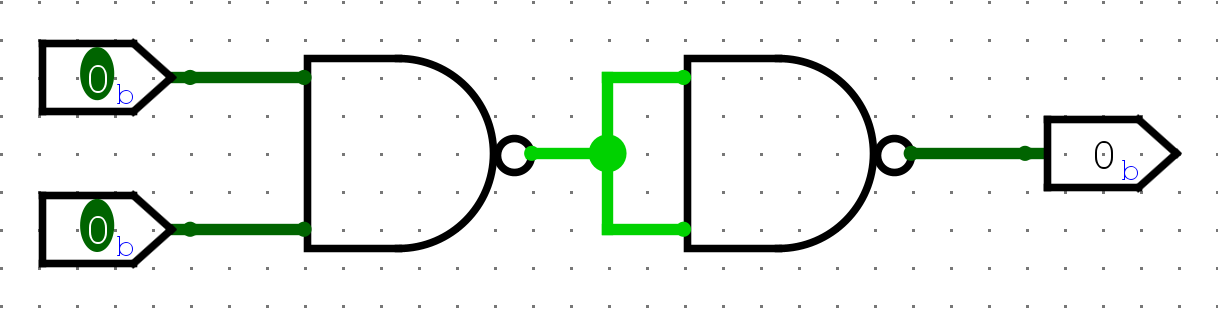
\includegraphics[width=0.75\textwidth]{./images/and_with_nand.png}
        \caption{AND Gate}
    \end{minipage}%
    \begin{minipage}{0.5\textwidth}
        \centering
        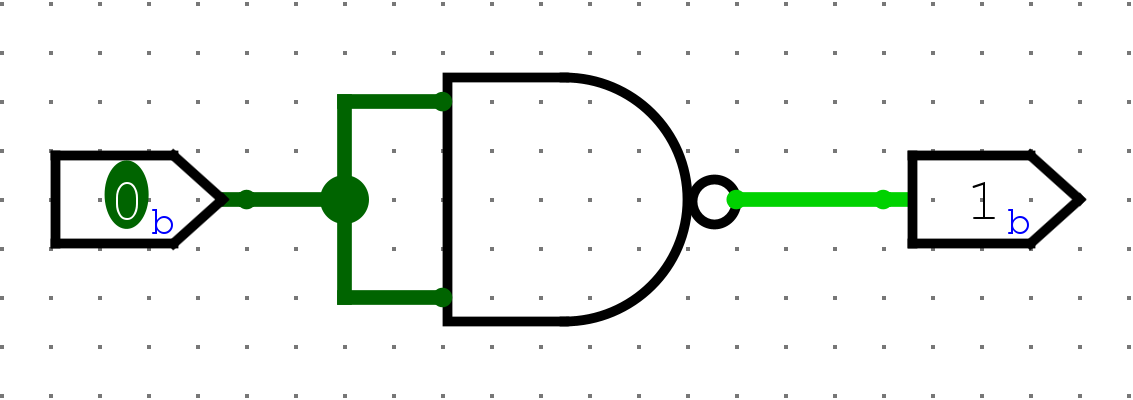
\includegraphics[width=0.75\textwidth]{./images/not_with_nand.png}
        \caption{NOT Gate}
    \end{minipage}
\end{figure}

\begin{figure}[H]
    \centering
    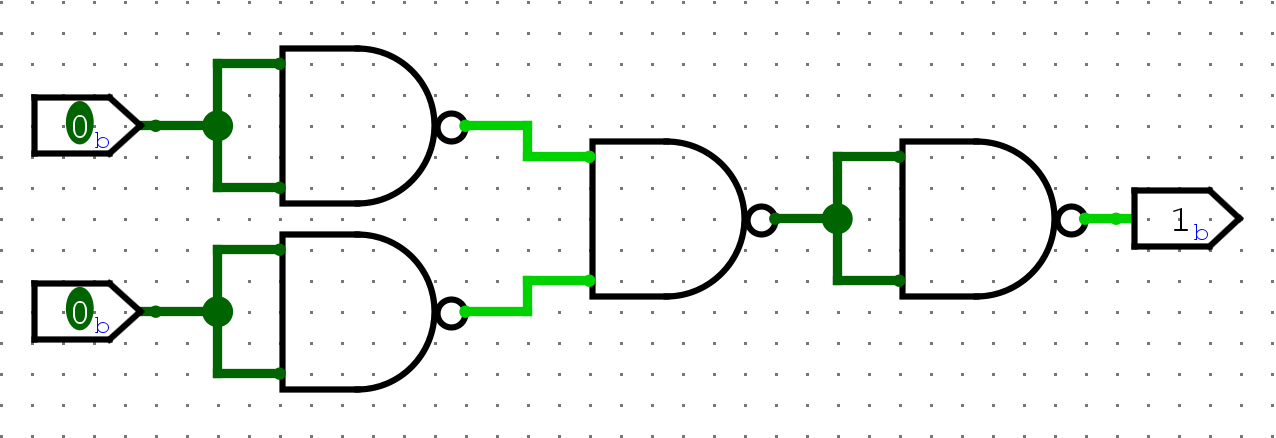
\includegraphics[width=0.5\textwidth]{./images/nor_with_nand.png}
    \caption{NOR Gate}
\end{figure}

\newpage
\section*{Problem 2}

\subsection*{Part A}
Electromechanical switches can be described by their number of poles and throws.
A pole is a common connection in a switch, and a throw is the number of positions the pole can connect to.
Therefore, a single-pole, single-throw (SPST) switch has one pole and one throw, which means it is just a simple on-off switch that connects or disconnects a single circuit.
The term NO means normally open, and it is used to describe the throw of a switch when it is not actuated (open means that the circuit is not connected).

\subsection*{Part B}
\begin{figure}[H]
    \centering
    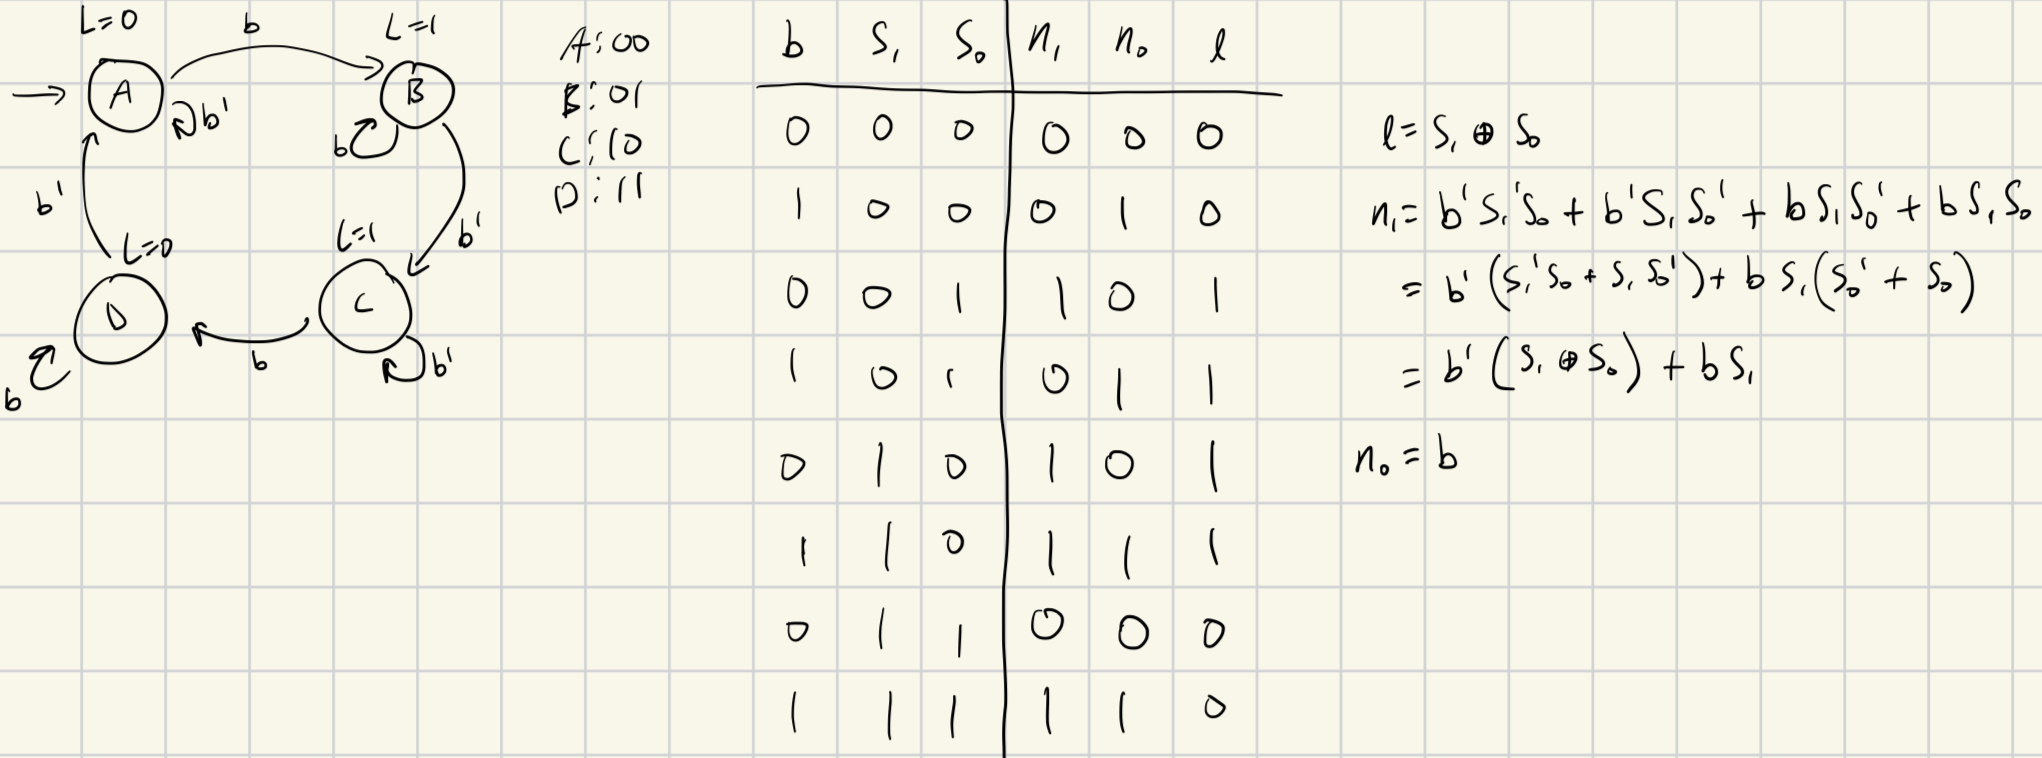
\includegraphics[width=\textwidth]{./images/problem2_plan.jpeg}
    \caption{FSM, Truth Table, and boolean expressions for the circuit}
\end{figure}

\subsection*{Part C}
\begin{figure}[H]
    \centering
    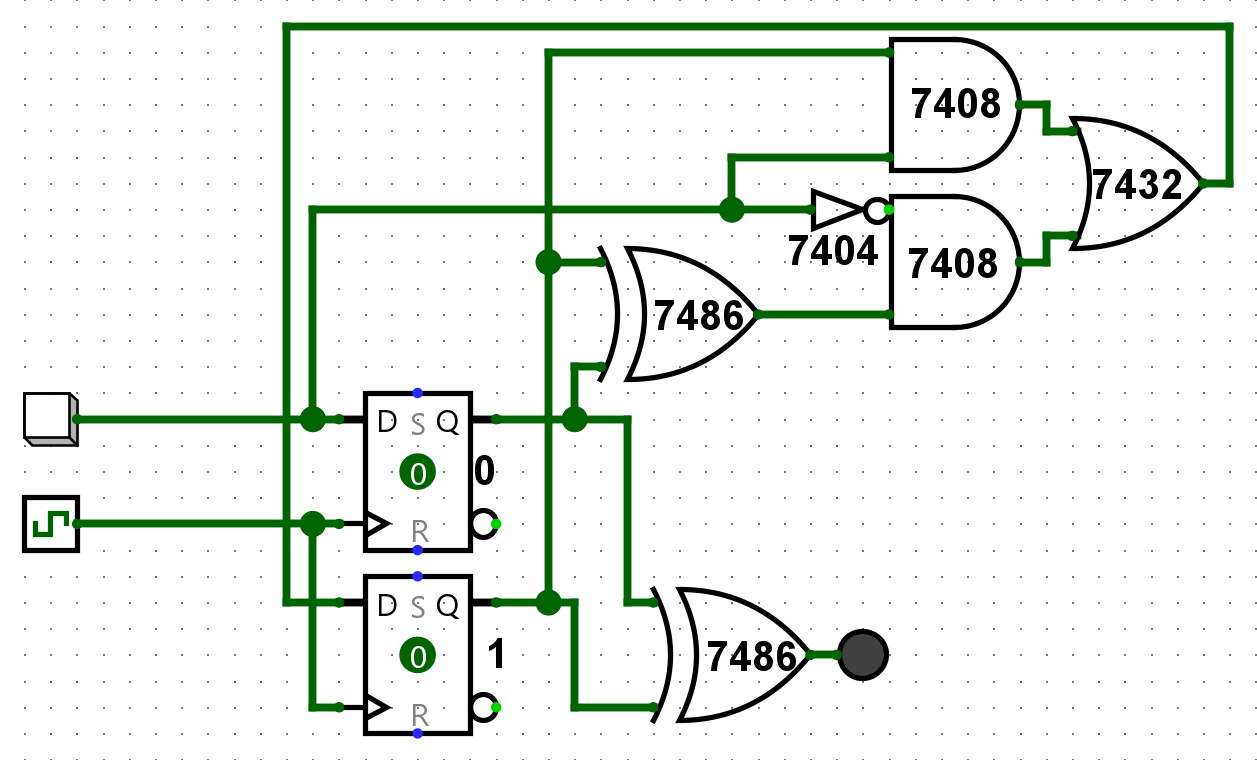
\includegraphics[width=0.75\textwidth]{./images/problem2_circ.png}
    \caption{Overall circuit with 74xx series equivalents}
\end{figure}

\newpage
\section*{Problem 3}

\subsection*{Part A}
\begin{figure}[H]
    \centering
    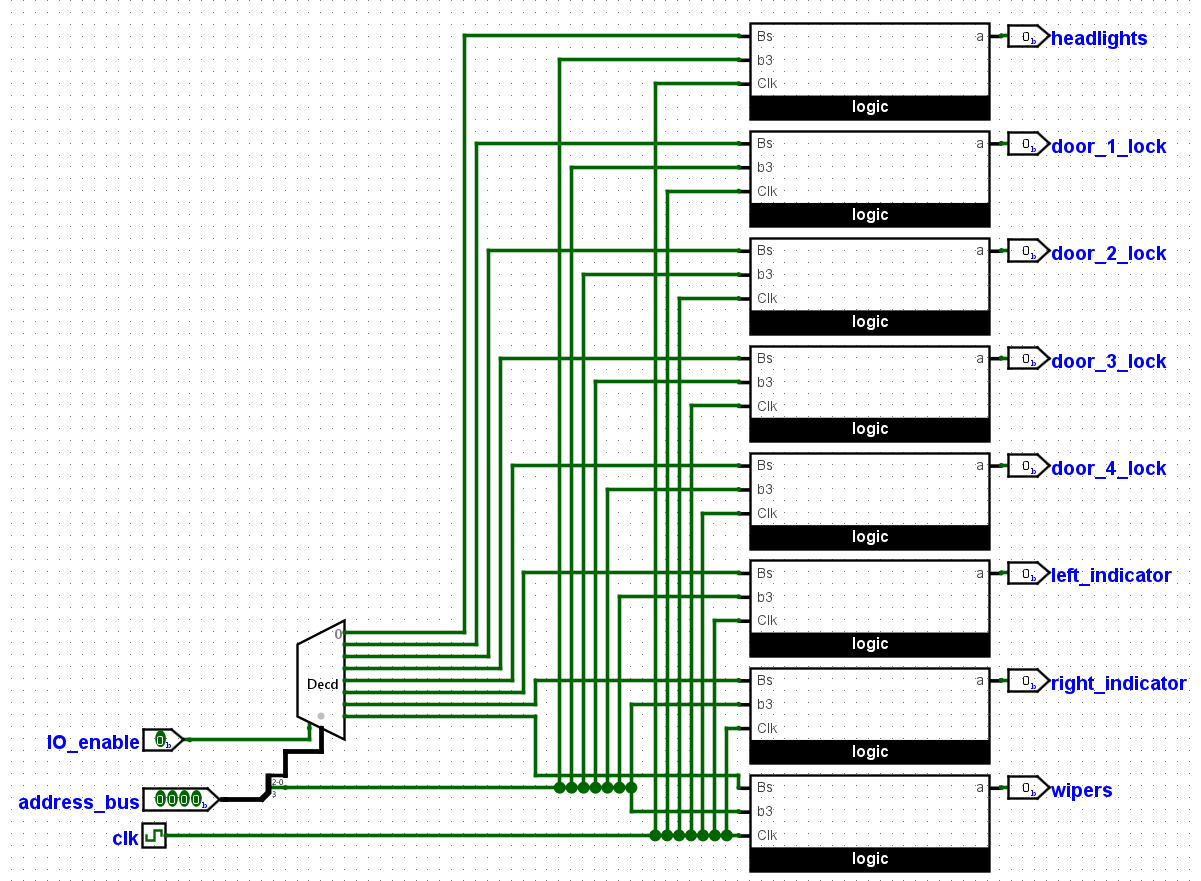
\includegraphics[width=\textwidth]{./images/problem3_circ1.png}
    \caption{Overall design of the circuit}
\end{figure}

\begin{figure}[H]
    \centering
    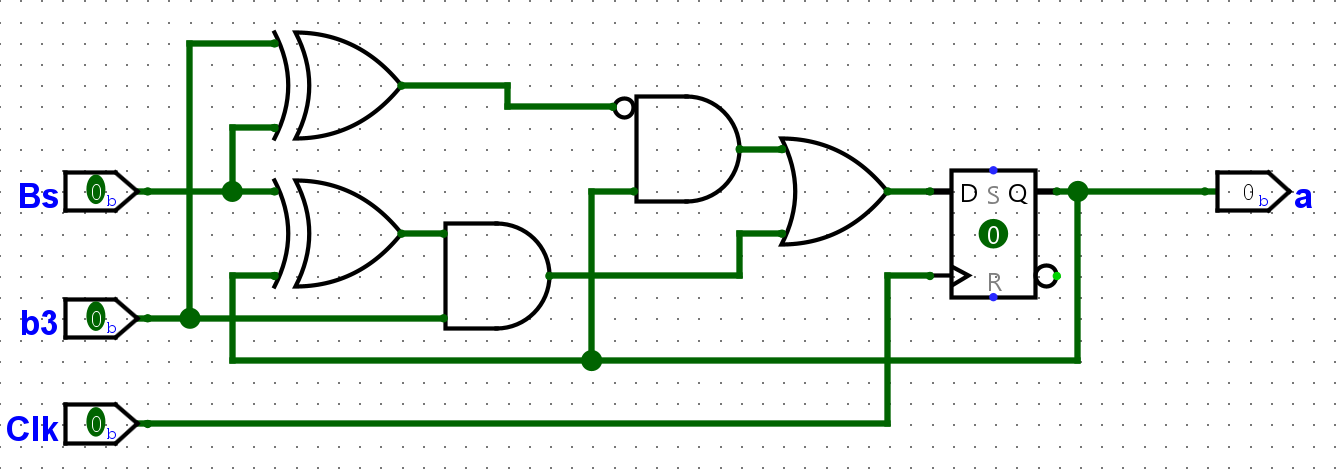
\includegraphics[width=0.75\textwidth]{./images/problem3_circ2.png}
    \caption{Logic implementation}
\end{figure}

\subsection*{Part B}
\begin{figure}[H]
    \centering
    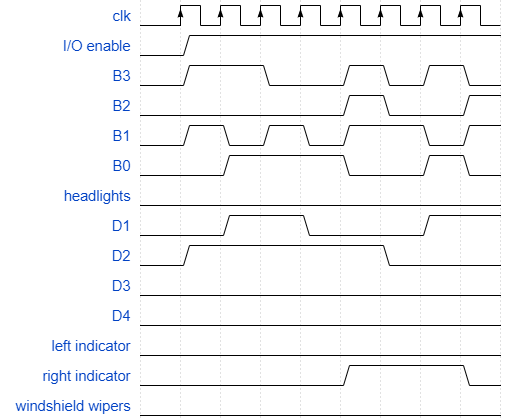
\includegraphics[width=0.75\textwidth]{./images/wavetable.png}
    \caption{Timing diagram}
\end{figure}

\end{document}
